%%%%%%%%%%%%%%%%%%%%%%%%%%%%%%%%%%%%%%%%%
% University Assignment Title Page 
% LaTeX Template
% Version 1.0 (27/12/12)
%
% This template has been downloaded from:
% http://www.LaTeXTemplates.com
%
% Original author:
% WikiBooks (http://en.wikibooks.org/wiki/LaTeX/Title_Creation)
%
% License:
% CC BY-NC-SA 3.0 (http://creativecommons.org/licenses/by-nc-sa/3.0/)
% 
% Instructions for using this template:
% This title page is capable of being compiled as is. This is not useful for 
% including it in another document. To do this, you have two options: 
%
% 1) Copy/paste everything between \begin{document} and \end{document} 
% starting at \begin{titlepage} and paste this into another LaTeX file where you 
% want your title page.
% OR
% 2) Remove everything outside the \begin{titlepage} and \end{titlepage} and 
% move this file to the same directory as the LaTeX file you wish to add it to. 
% Then add \documentclass[12pt]{article}
\usepackage[english]{babel}
\usepackage{amsmath}
\usepackage{graphicx}
\usepackage{textcomp}
\usepackage{parskip}
\usepackage[colorinlistoftodos]{todonotes}
\usepackage{csquotes}
\usepackage{float}
\usepackage[backend=biber,style=ieee]{biblatex}
\addbibresource{bibliography.bib}

\begin{document}

\begin{titlepage}

\newcommand{\HRule}{\rule{\linewidth}{0.5mm}}
\center 

\textsc{\LARGE Iowa State University }\\[1.5cm] 
\textsc{\Large Center for Statistics and Applications in Forensic
Evidence
}\\[0.5cm] 

\HRule \\[0.4cm]
{ \huge \bfseries Shoe Print Data Collection: Additional Methods }\\[0.4cm] 
\HRule \\[1.5cm]



\begin{center}
\centering
 
\includegraphics[scale=.4]{csafe-logo}\\[1cm]
\end{center}







\end{titlepage}

\section{Introduction}

 When developing the methodology for the longitudinal shoe study conducted by the Center for Statistics and Applications in Forensic Evidence (CSAFE), collection procedures were designed to obtain the most ideal shoe-sole impression possible. While these images will be useful to the researcher and practitioner communities, they do not provide realistic examples of prints that would be collected from a crime scene/suspected crime scene. For this reason, CSAFE researchers have compiled this manual which contains procedures for further data collection and offers new, or edited, procedures that better represent the practices of current forensic examiners and crime scene teams. If at any time there is a question on any of these procedures, please make a note using a post-it note and e-mail the principal investigator, the project manager, the faculty in charge of the study, or the author of the specific procedure. 

\end{document} to your LaTeX file where you want your
% title page.
%
%%%%%%%%%%%%%%%%%%%%%%%%%%%%%%%%%%%%%%%%%
%\title{Title page with logo}
%----------------------------------------------------------------------------------------
%	PACKAGES AND OTHER DOCUMENT CONFIGURATIONS
%----------------------------------------------------------------------------------------

\documentclass[12pt]{article}
\usepackage[english]{babel}
\usepackage[utf8x]{inputenc}
\usepackage{amsmath}
\usepackage{graphicx}
\usepackage[colorinlistoftodos]{todonotes}

\begin{document}

\begin{titlepage}

\newcommand{\HRule}{\rule{\linewidth}{0.5mm}} % Defines a new command for the horizontal lines, change thickness here

\center % Center everything on the page
 
%----------------------------------------------------------------------------------------
%	HEADING SECTIONS
%----------------------------------------------------------------------------------------

\textsc{\LARGE Iowa State University}\\[1.5cm] % Iowa State University 
\textsc{\Large CSAFE}\\[0.5cm] % CSAFE
\textsc{\large Center for Statistics and Applications in Forensic Evidence }\\[0.5cm] % Center for Statistics and Applications in Forensic Evidence 

%----------------------------------------------------------------------------------------
%	2D Shoe Scanner Procedure
%----------------------------------------------------------------------------------------

\HRule \\[0.4cm]
{ \huge \bfseries EinScan Pro+ 3D Scanner: Procedure (Phase 2)  }\\[0.4cm] % Title of your document
\HRule \\[1.5cm]
 
%----------------------------------------------------------------------------------------
%	AUTHOR SECTION
%----------------------------------------------------------------------------------------

\begin{minipage}{0.4\textwidth}
\begin{flushleft} \large
\emph{Author:}\\
\textsc{James E. Kruse} % James E. Kruse
\end{flushleft}
\end{minipage}
~
\begin{minipage}{0.4\textwidth}
\begin{flushright} \large
\emph{Supervisor:} \\
\textsc{Dr. Guillermo Basulto-Elias} % Supervisor's Name
\end{flushright}
\end{minipage}\\[2cm]

%----------------------------------------------------------------------------------------
%	LOGO SECTION
%----------------------------------------------------------------------------------------

\includegraphics[scale=.5]{Logo}\\[1cm]

\begin{center}
\begin{tabular}{ c   |   c } 
 
\end{tabular}
\end{center}
%----------------------------------------------------------------------------------------
%	DATE SECTION
%----------------------------------------------------------------------------------------

{\large \today}\\[2cm] % Date, change the \today to a set date if you want to be precise


%----------------------------------------------------------------------------------------

\vfill % Fill the rest of the page with whitespace

\end{titlepage}




\section{Introduction}

The following is the recommended procedure for using the EINSCAN Pro+ 3D scanner (Figure 1). While it is not the primary purpose of this devise, it will be used to create 3D, digital models of shoe soles. 

This method is different from that used during phase 1 of the longitudinal shoe data collection project. New equipment is implemented in this procedure and a better quality model is obtained as an end product. 

\begin{figure}[!htp]
\centering
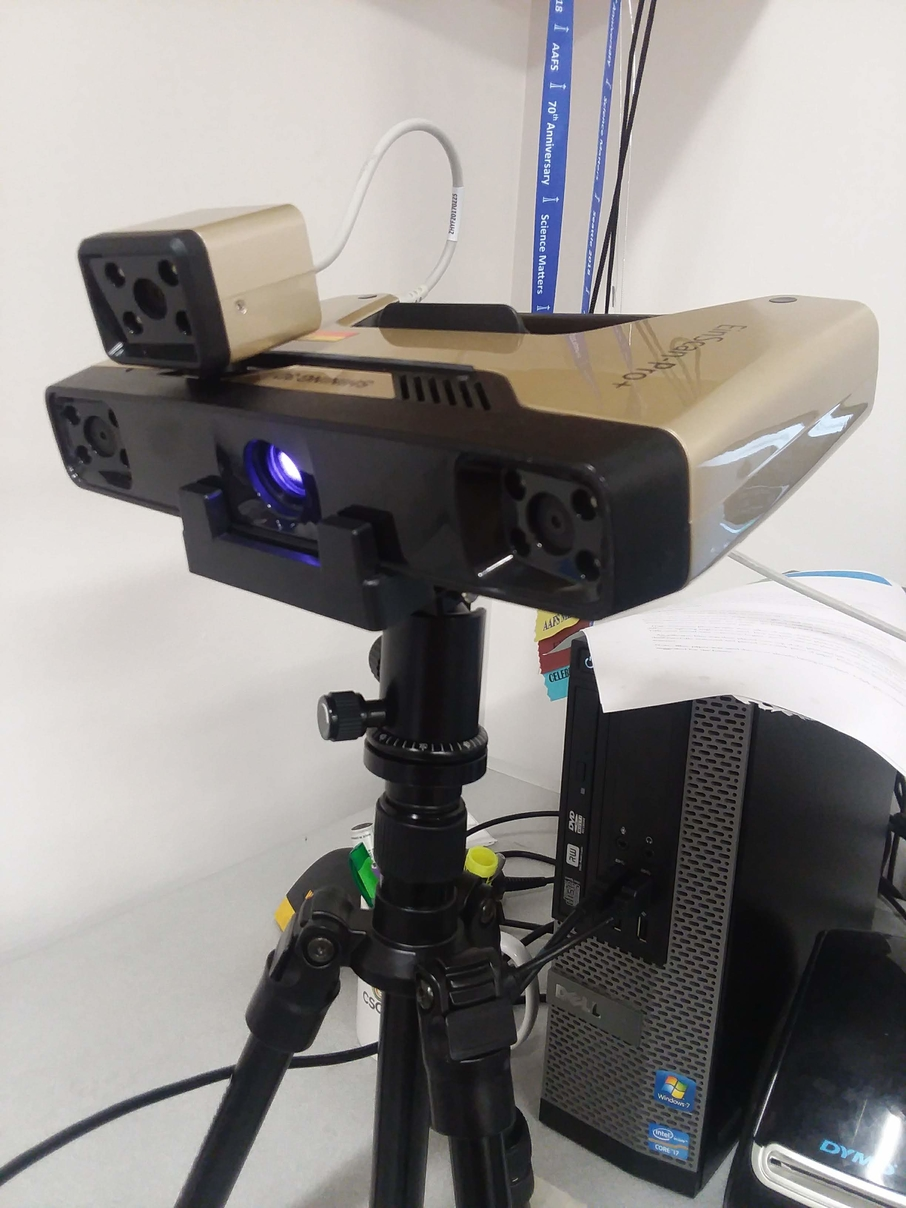
\includegraphics[width=4cm]{Scanner}
\caption{EinScan Pro+}
\label{Image 1}
\end{figure}


\subsection{Procedure}

1.	Prior to use, contact IT to install the necessary software in the desired computer. Make sure all cords for the EINSCAN Pro+ are connected to both the scanner itself and to the computer. There will be a gray USB that will connect directly into the computer and a black power chord that will plug into the hub on the USB (Figure 2). This black cord will provide power to the scanner. 

\begin{figure}[!htp]
\centering
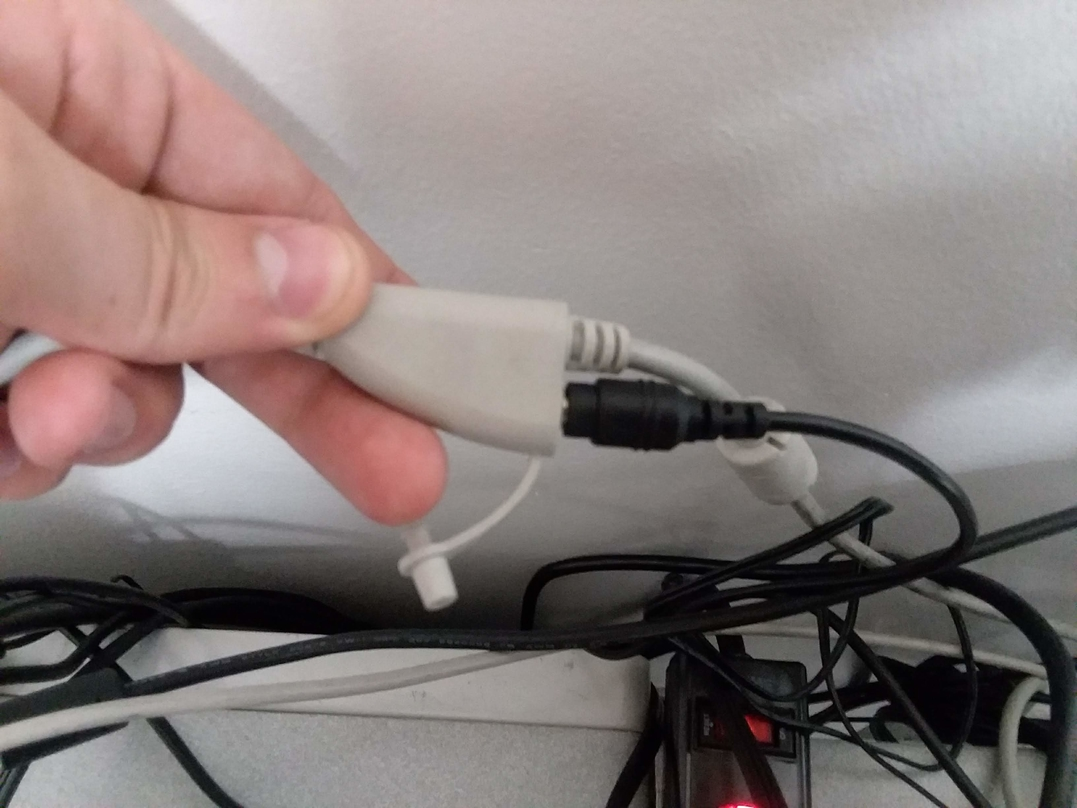
\includegraphics[width=5cm]{Plug}
\caption{Insert the black power cord into the hub on the USB cord.}
\label{Image 2}
\end{figure}

\newpage

2. On the desk, near the back wall of the shoe office, the exact location of all equipment is marked with spike tape. Place the box for the 3D scanner in its marked place (Figure 3). 

\begin{figure}[!htp]
\centering
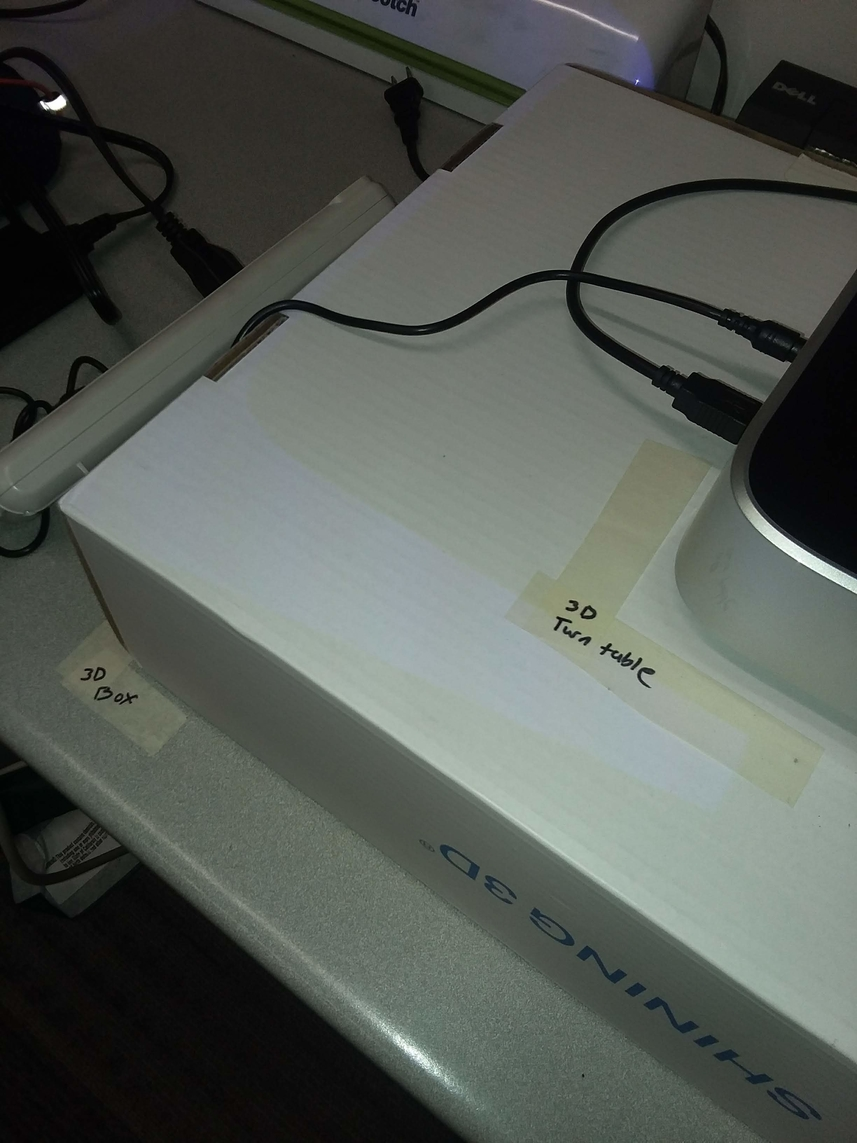
\includegraphics[width=4cm]{Spike_Turn_Table}
\caption{The spike marks for the box are on the desk while those for the turn table on on the box.}
\label{Image 3}
\end{figure}


3. Obtain the "Shining 3D" turn table and place it in its marked place, on the 3D Scanner box (Figure 3). There will be two black cords that came with the turntable. The first will have a USB on one end and a connector for the turntable on the other. plug the connector into the turntable and the USB into the computer. Secondly, connect the black power cord to the turntable and then into the wall. A power strip may be necessary to reach an outlet. 

\newpage

4. Obtain the miniature tripod that came with the turntable. The legs and neck of the tripod will not need to be extended. Simply position the legs so they match the labeled spike marks on the desk (Figure 4). 

\begin{figure}[!htp]
\centering
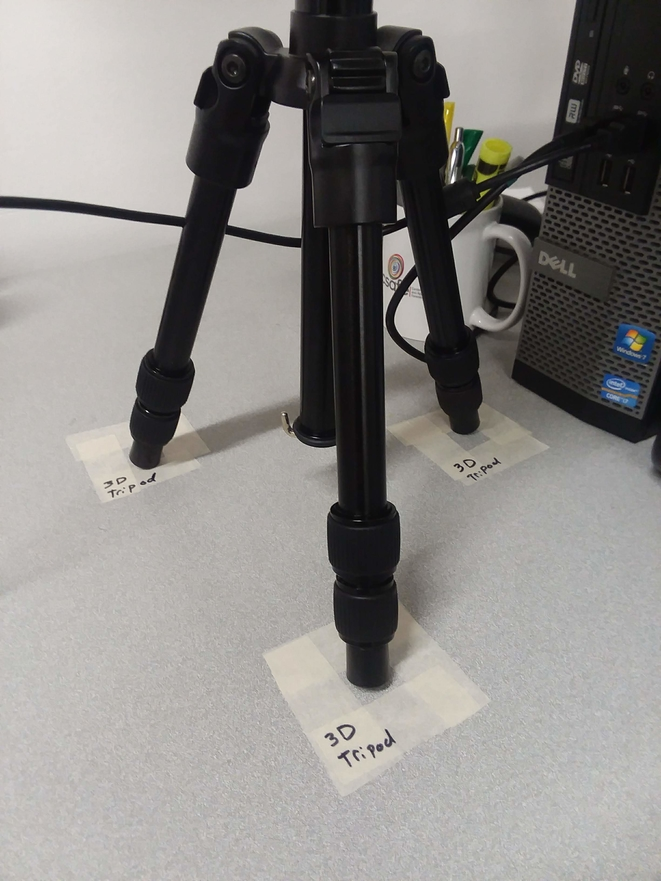
\includegraphics[width=4cm]{Spike_Tripod}
\caption{There will be three spike marks for the tripod legs}
\label{Image 4}
\end{figure}

5. Attach the scanner mount to the tripod (Figure 5). Once secure, position the scanner in the mount and make sure that all weight is balanced (Figure 6). 

\begin{figure}[!htp]
\centering
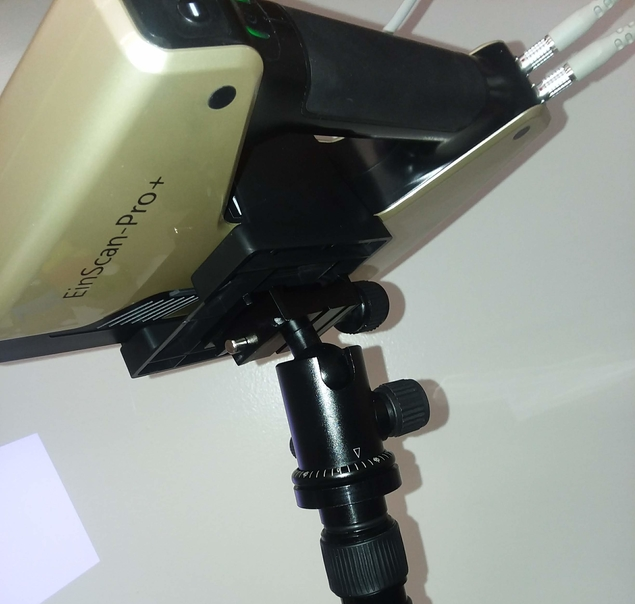
\includegraphics[width=4cm]{Clip}
\caption{Position the scanner securely into the mount}
\label{Image 5}
\end{figure}

\begin{figure}[!htp]
\centering
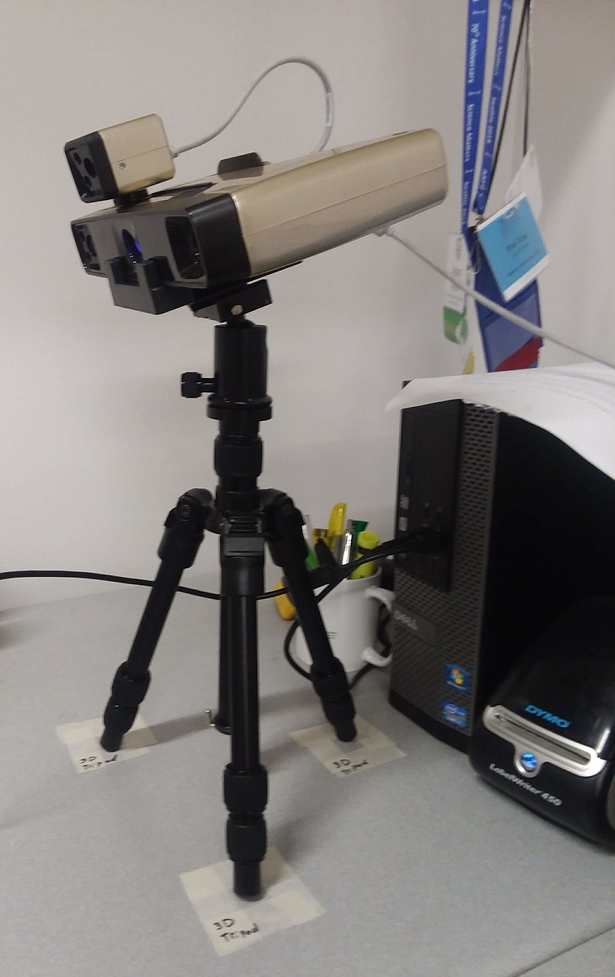
\includegraphics[width=4cm]{Full_Tripod}
\caption{The final scanner set-up.}
\label{Image 6}
\end{figure}

\newpage

6. Launch the EinScan Pro program located on the desktop (Figure 7). Select "EinScan Pro+" (Figure 8) . 
 
 \begin{figure}[!htp]
\centering

\includegraphics[width=2cm]{Icon}
\caption{Desktop icon to launch the Program}
\label{Image 7}
\end{figure}

\begin{figure}[!htp]
\centering
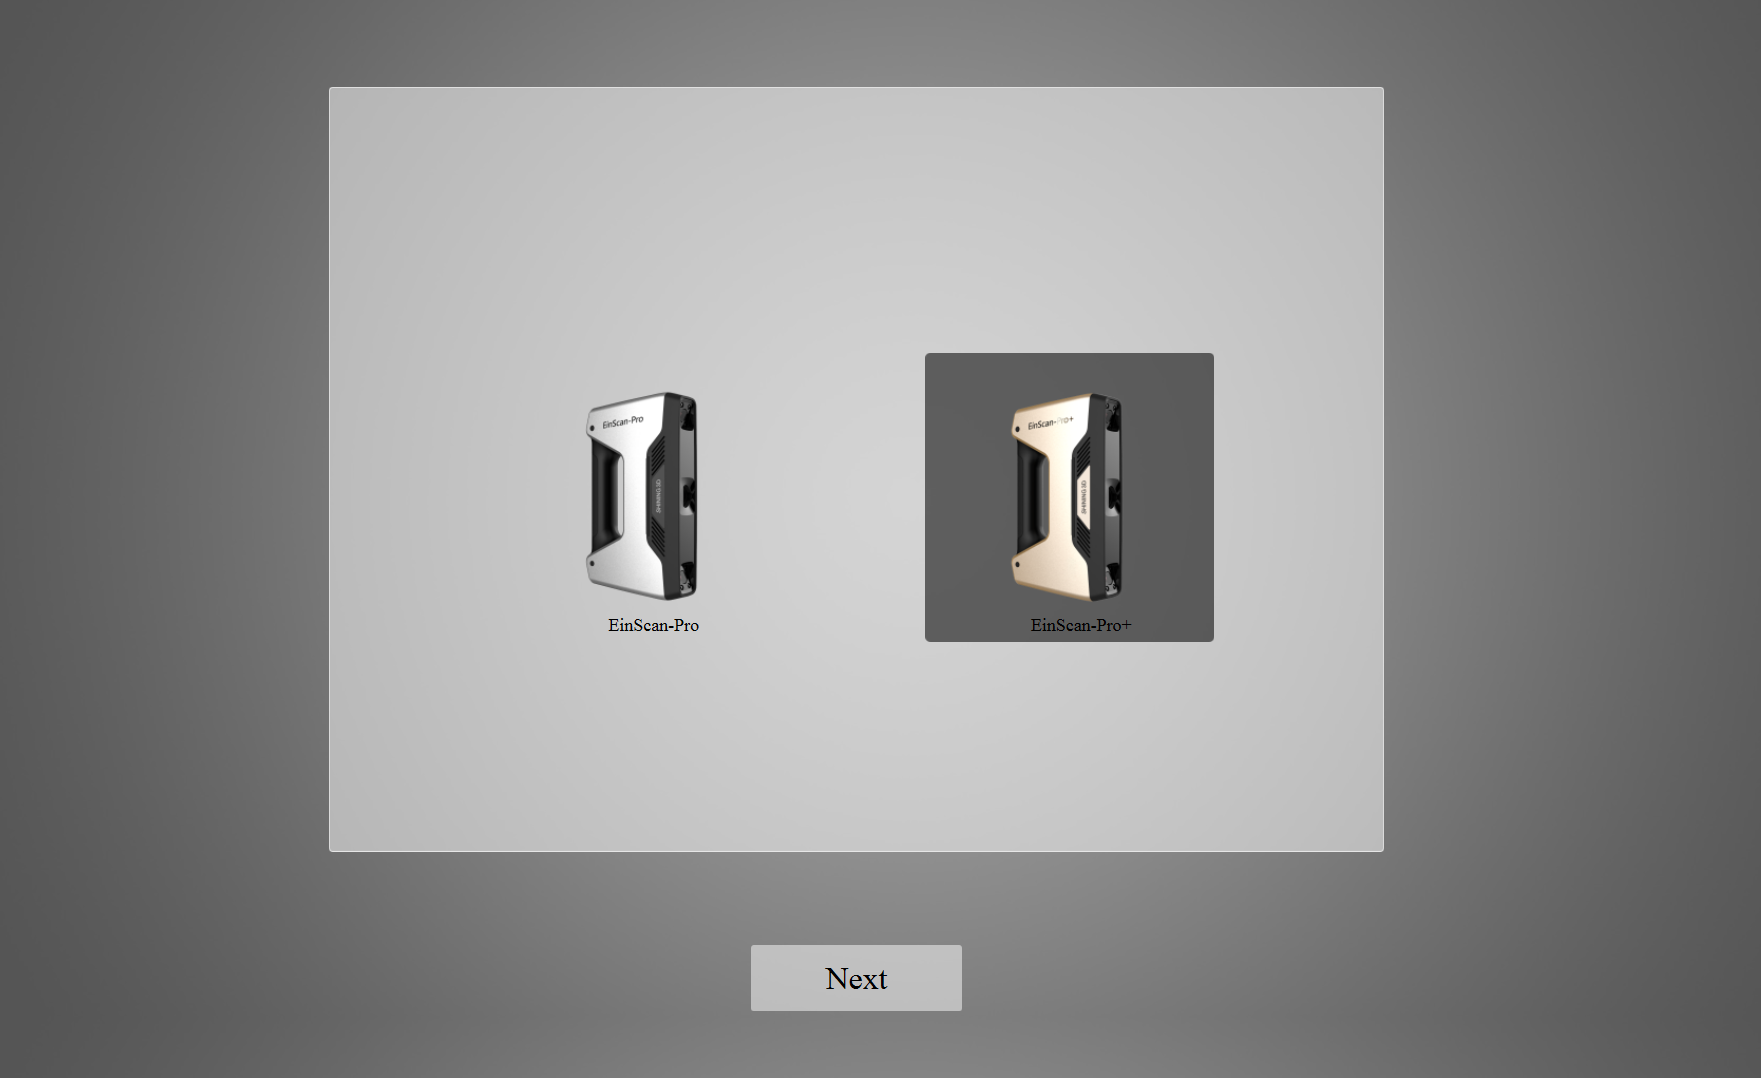
\includegraphics[width=6cm]{Home_Screen}
\caption{Select EinScan Pro+}
\label{Image 8}
\end{figure}

\newpage

7. Select "Fixed Scan Mode" (Figure 9) and select the project plan you desire. In most cases, you will create a new project. (Figure 10). 

\begin{figure}[!htp]
\centering
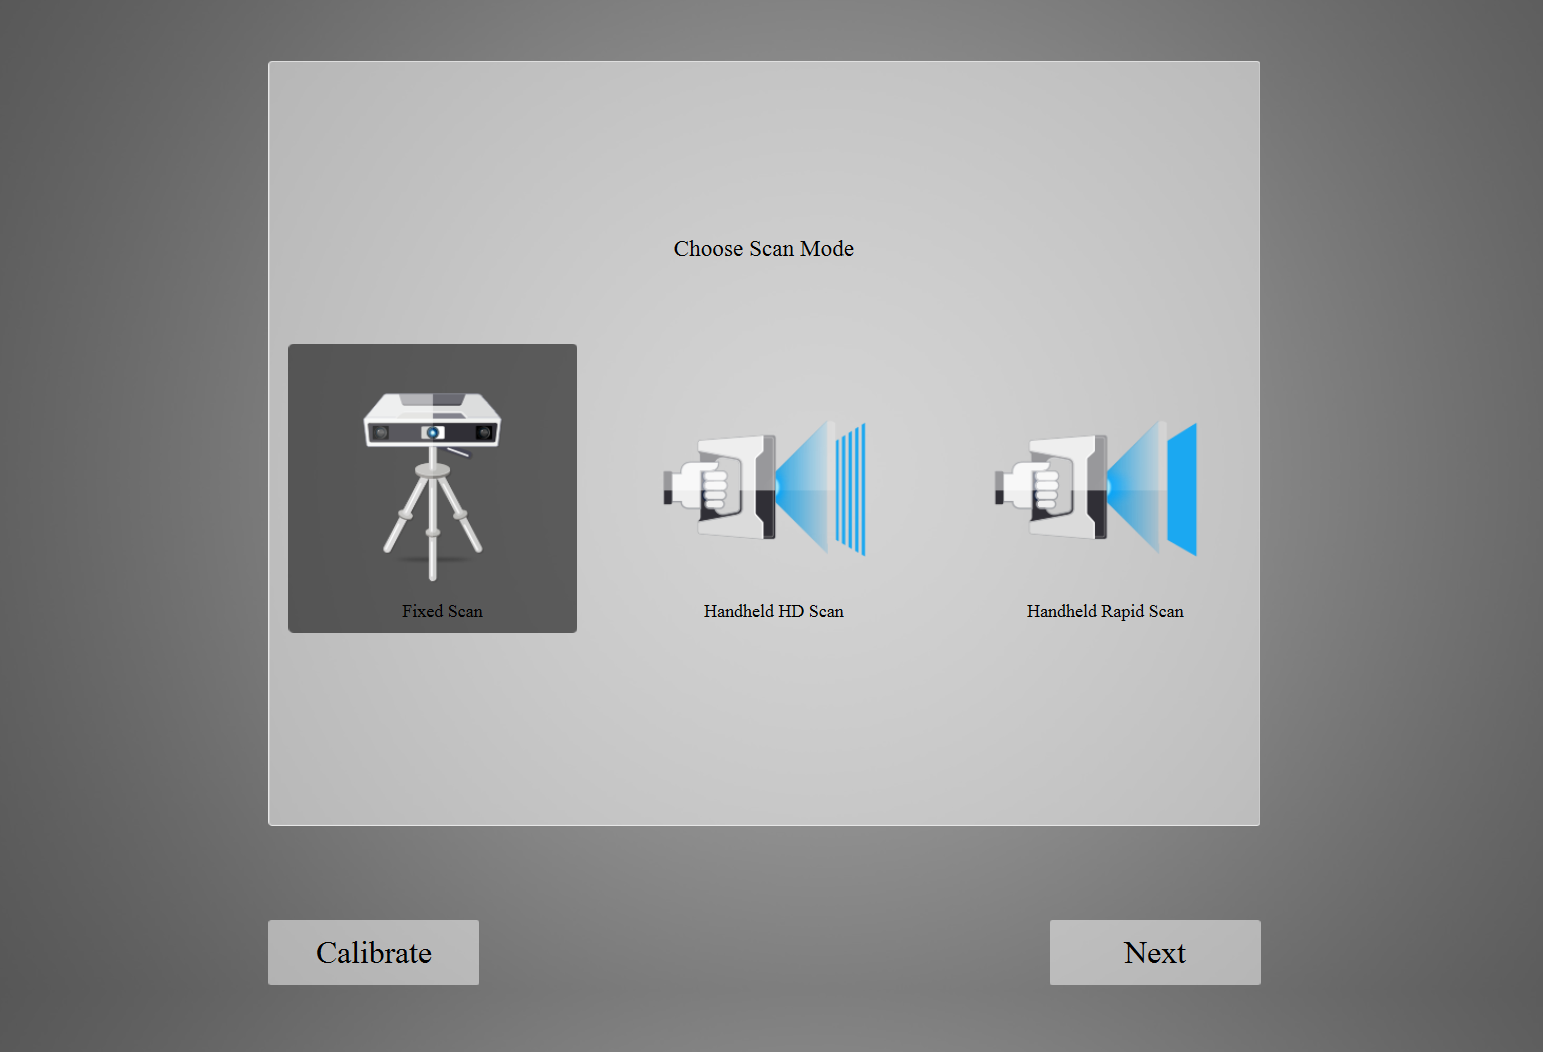
\includegraphics[width=6cm]{Choose}
\caption{Select "Fixed Scan Mode"}
\label{Image 9}
\end{figure}

\begin{figure}[!htp]
\centering
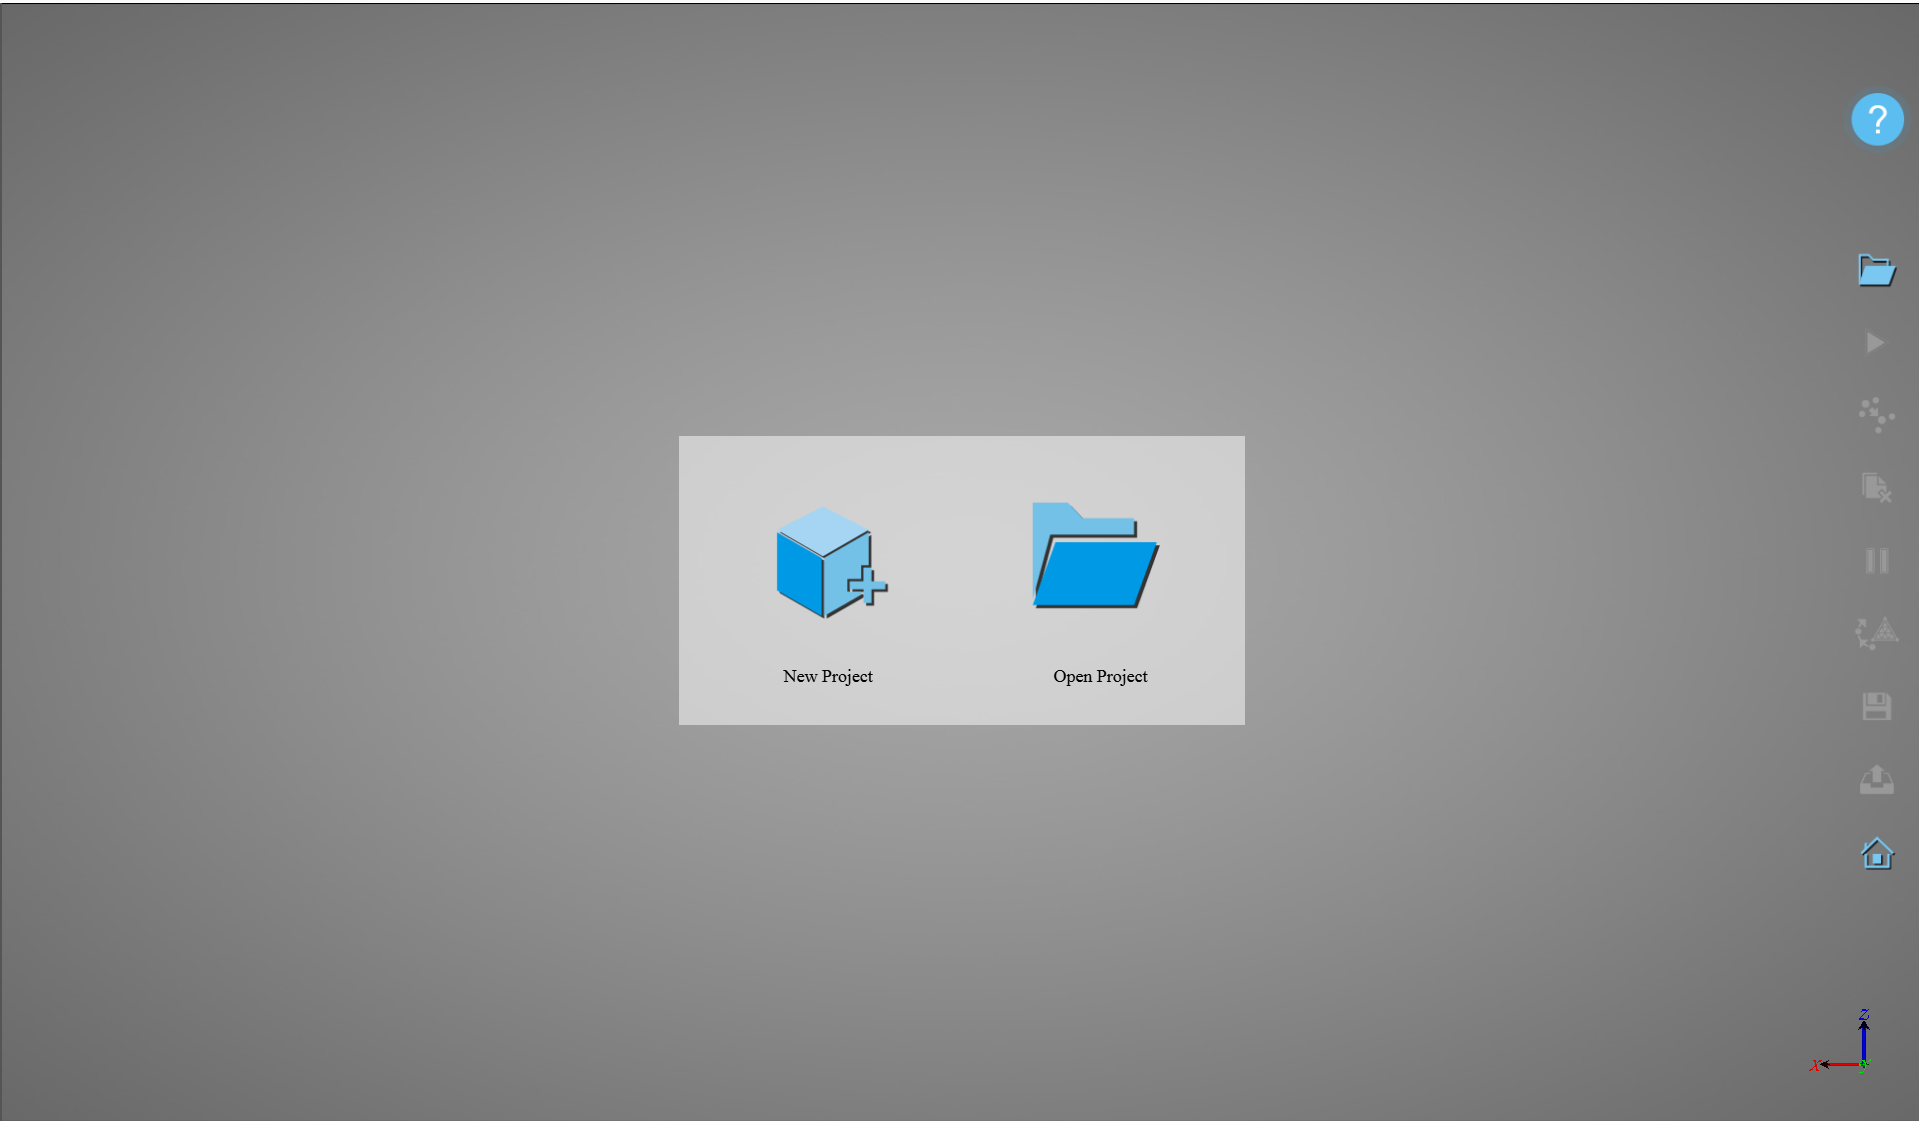
\includegraphics[width=6cm]{New_Project}
\caption{Project Selection}
\label{Image 10}
\end{figure}

8. Select "Non-Texture Scan" (Figure 11). Finish by selecting "Apply".

\begin{figure}[!htp]
\centering
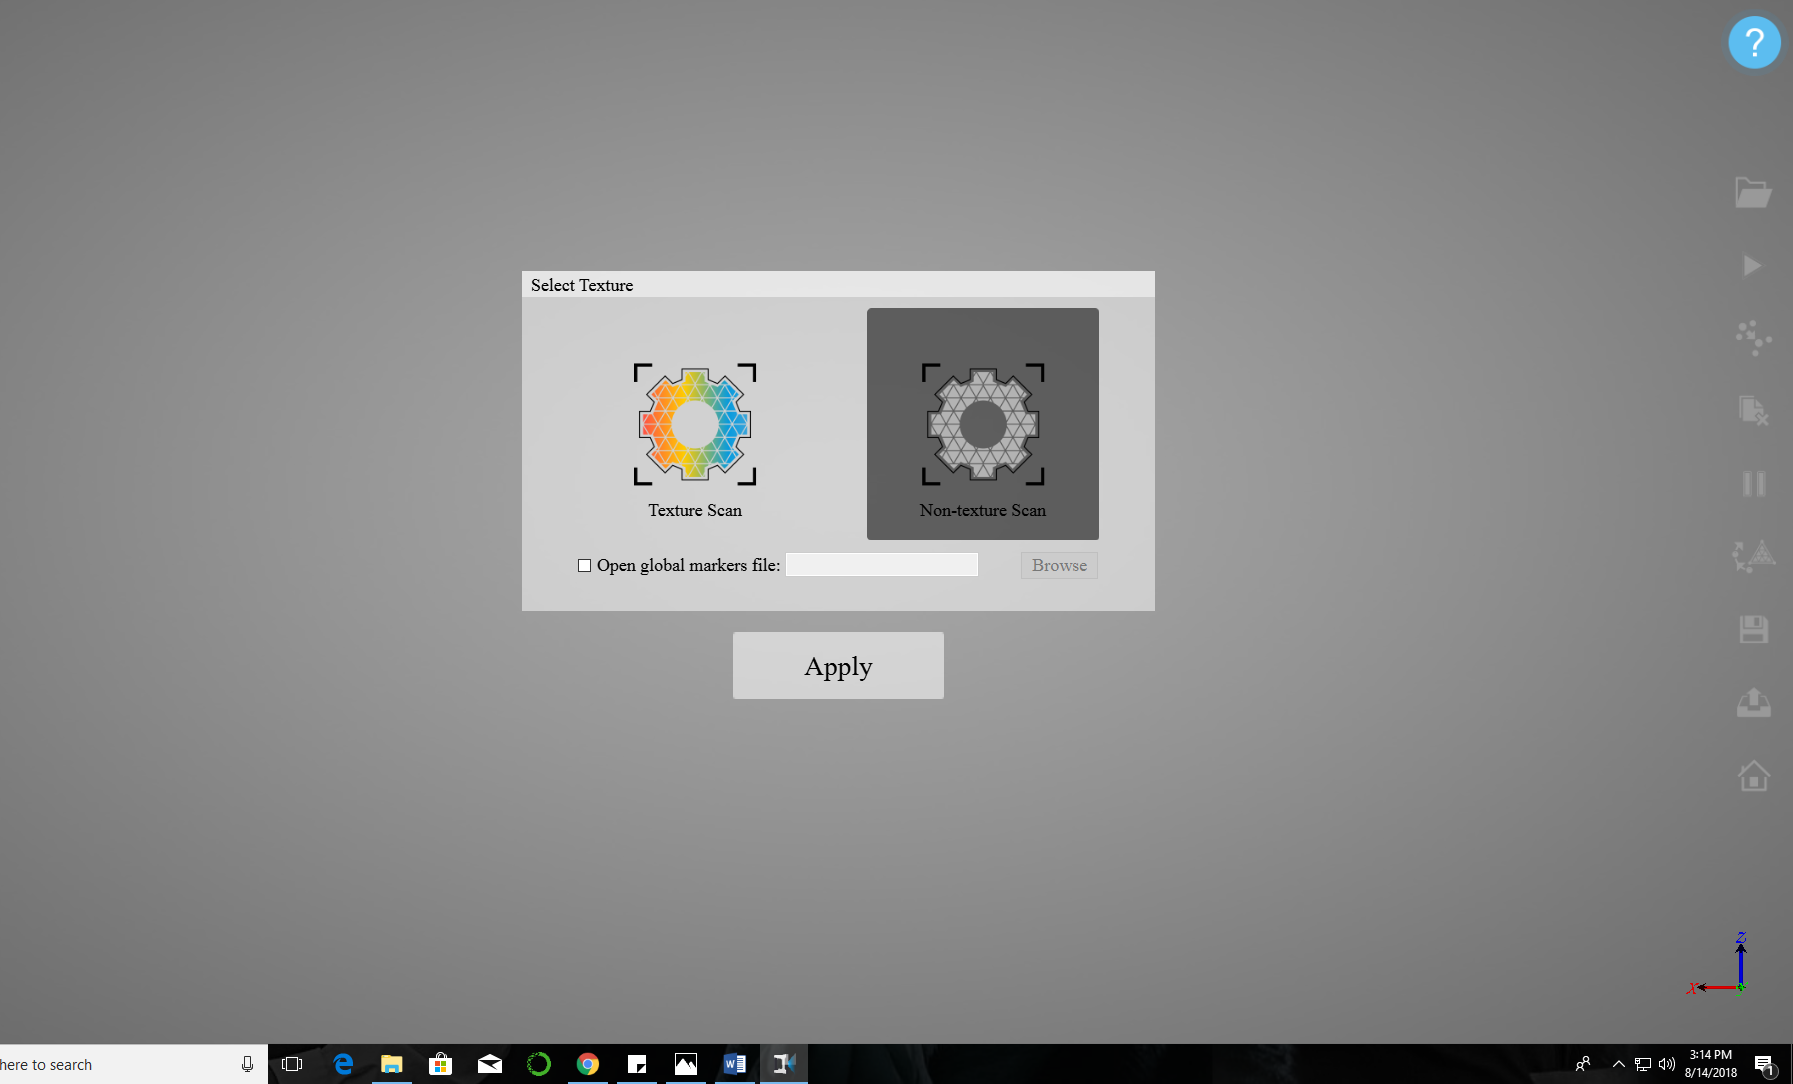
\includegraphics[width=6cm]{Color}
\caption{Select "Non-Texture Scan"}
\label{Image 11}
\end{figure}

\newpage

9. Place the Shoe onto the turntable with the sole facing the scanner (Figure 12). You will want to make sure that the laces and all other pieces are tucked. No part of the shoe should be hanging off of the turn table. The scanner will project a cross onto the shoe to make sure everything is centered (Figure 13). 

\begin{figure}[!htp]
\centering
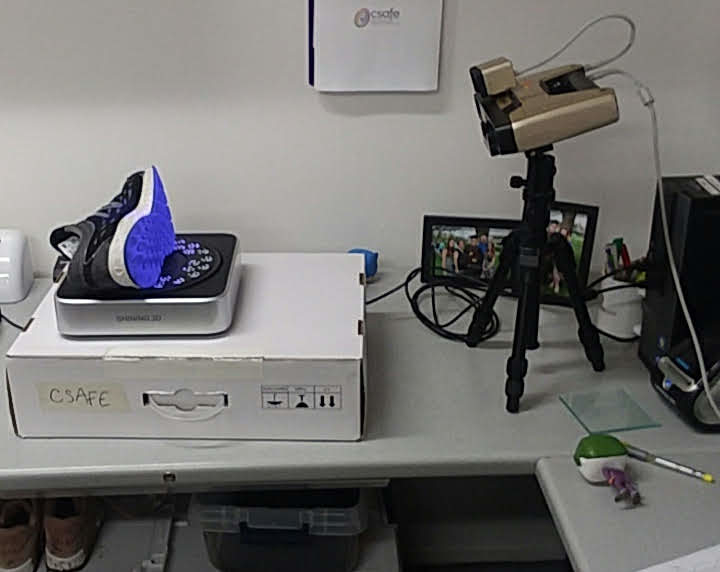
\includegraphics[width=6cm]{Full}
\caption{The Complete set-up for the 3D scanner and turn table.}
\label{Image 12}
\end{figure}

\begin{figure}[!htp]
\centering
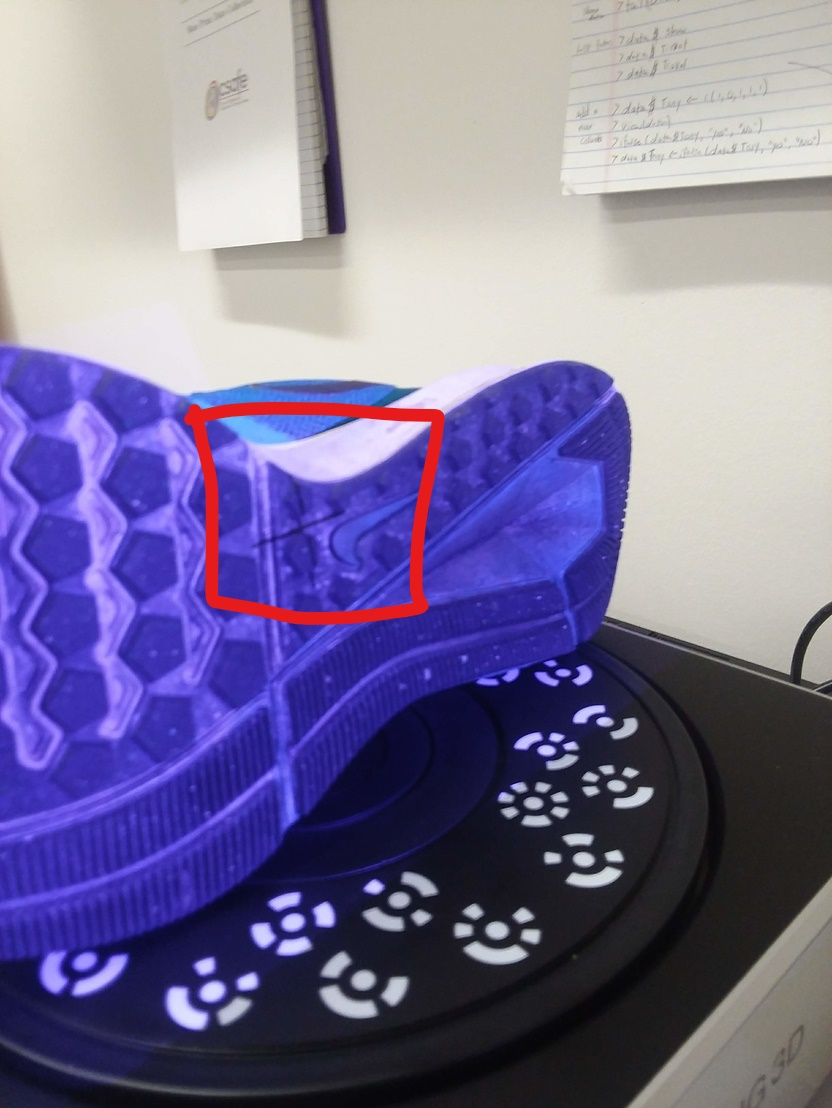
\includegraphics[width=4cm]{Cross_on_Shoe_LI}
\caption{For a good scan, the cross should be centered in the shoe.}
\label{Image 13}
\end{figure}

10. Locate the brightness setting and select level 2 (Figure 14). This will allow the scanner to pick up on the finer details of the shoe. On this level there will be relatively little red on the live screen (Figure 15)

\begin{figure}[!htp]
\centering

\includegraphics[width=6cm]{Brightness_Bar}
\caption{Brightness Level 2}
\label{Image 14}
\end{figure}

\begin{figure}[!htp]
\centering
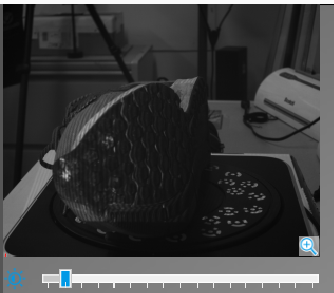
\includegraphics[width=6cm]{Live}
\caption{The live screen will display the shoe as the scanner can see it.}
\label{Image 15}
\end{figure}

\newpage

11. Below the brightness bar, the technician will then select "With Turntable". Enter 15 for "Turn Table Steps". Under "Align Mode", select "Feature" (Figure 16).

\begin{figure}[!htp]
\centering
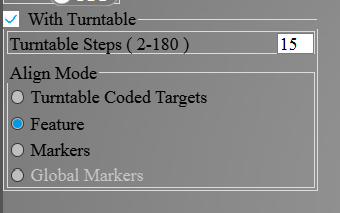
\includegraphics[width=6cm]{Turn_Table_Mode}
\caption{All turntable setting should match those in this image.}
\label{Image 16}
\end{figure}

12. At this point, all settings should be correct. Select the play button located on the far left tool bar (Figure 17). At that point the scanner will begin verifying the object (Figure 18). The scan will begin if all settings and placements are correct. If verification fails, please review previous steps to make sure all settings and locations are correct.


\begin{figure}[!htp]
\centering
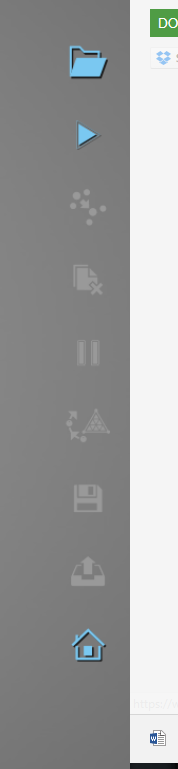
\includegraphics[width=2cm]{Tool_Bar_1}
\caption{The play button is second from the top.}
\label{Image 17}
\end{figure}


\begin{figure}[!htp]
\centering
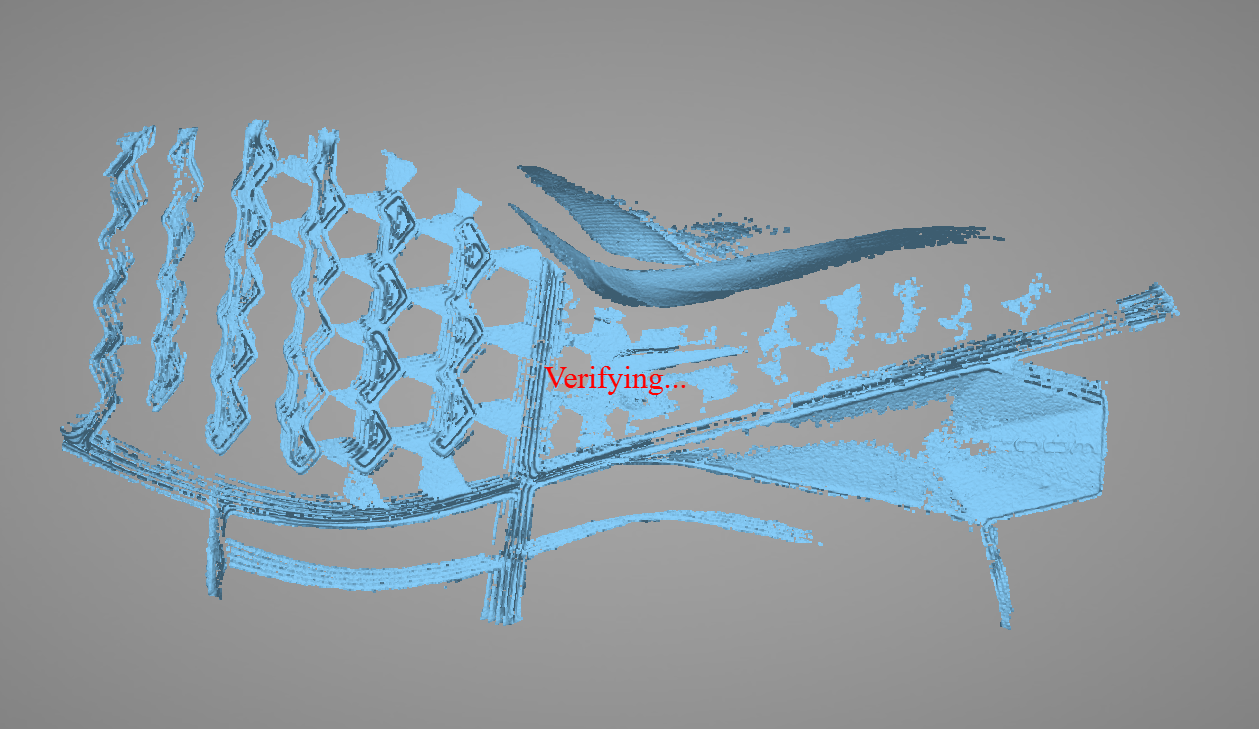
\includegraphics[width=7cm]{Ver}
\caption{The scanner will run a test to see of all objects are in their correct place and if all settings are correct.}
\label{Image 18}
\end{figure}

\newpage

13. As the scanner runs, it will appear that the system is missing most of the shoe. That is OK. Keep an eye on the turntable and the screen to make sure that at no point the scan fails.  

14. At the end of the scan, the scan will center on the screen (Figure 19) and the technician will either have to approve or deny the scan (Figure 20). The scan can be maneuvered to look over all points. Keep in mind that brightness level two will not capture the majority of the shoe. If the scan needs to be repeated, select the red "X". If everything is satisfactory, select the green check.  

\begin{figure}[!htp]
\centering
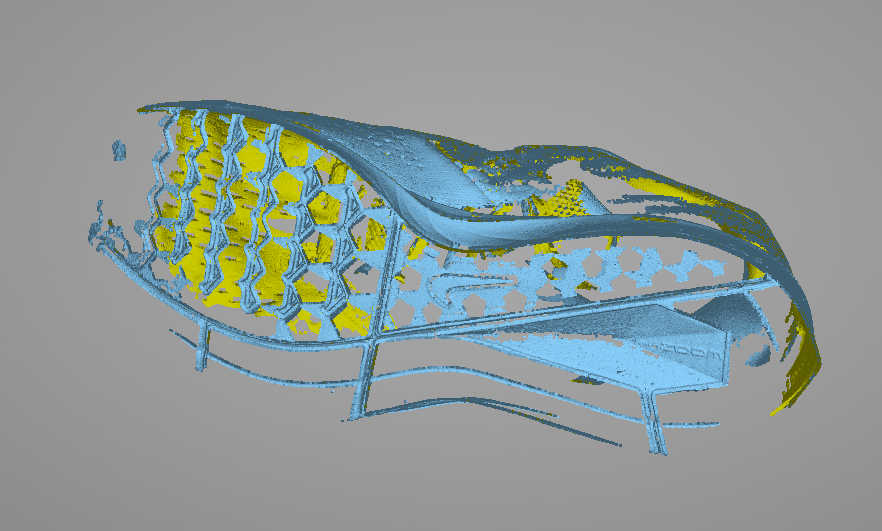
\includegraphics[width=6cm]{2}
\caption{Final image when scanned on brightness level 2.}
\label{Image 19}
\end{figure}

\begin{figure}[!htp]
\centering
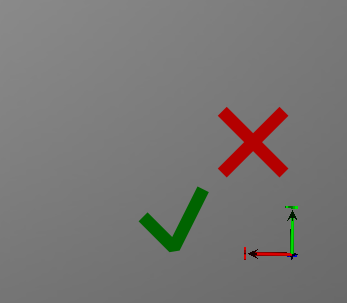
\includegraphics[width=6cm]{YesNo}
\caption{Approve or deny the initial model}
\label{Image 20}
\end{figure}

15. At this point, do not move the shoe. Adjust the brightness to level 8 (Figure 21) and re-run the scan. This will pick up on the rest of the details. At the conclusion of the scan, once again, either approve or deny the scan.

\begin{figure}[!htp]
\centering

\includegraphics[width=6cm]{Brightness_Bar_8}
\caption{Adjust the brightness bar to level 8.}
\label{Image 21}
\end{figure}

16. If there are any portions of the shoe missing at this point, adjust the shoe and re-run the scan (Step 15). If there continues to be problems, try adjusting the brightness. 

17. Once all scans have been completed, the program will have combined all images into one . If the program did not line up the images properly, delete the scan and start the procedure over. 

18. If there are pieces in the scan that are not part of the shoe, they will need to be removed. hold down the select key on the keyboard and trace the artifact with the mouse (Figure 22). This will turn the item red. After all items have been selected, select the trash can on the bottom of the screen (Figure 23). 

\begin{figure}[!htp]
\centering
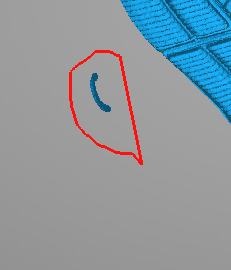
\includegraphics[width=6cm]{Mark}
\caption{Select the artifact and it will turn red.}
\label{Image 22}
\end{figure}

\begin{figure}[!htp]
\centering

\includegraphics[width=6cm]{Second_Tool_Bar}
\caption{Select the trash can after all artifacts have been selected.}
\label{Image 23}
\end{figure}

\newpage

19. At this point, the final rough scan has been completed (Figure 24-25).

\begin{figure}[!htp]
\centering
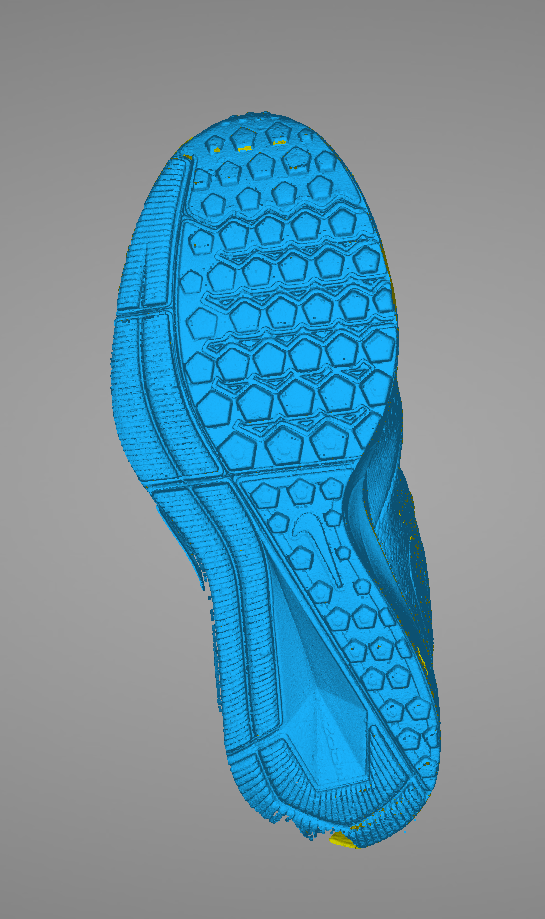
\includegraphics[width=5cm]{Shoe}
\caption{Final Rough Scan}
\label{Image 24}
\end{figure}

\begin{figure}[!htp]
\centering
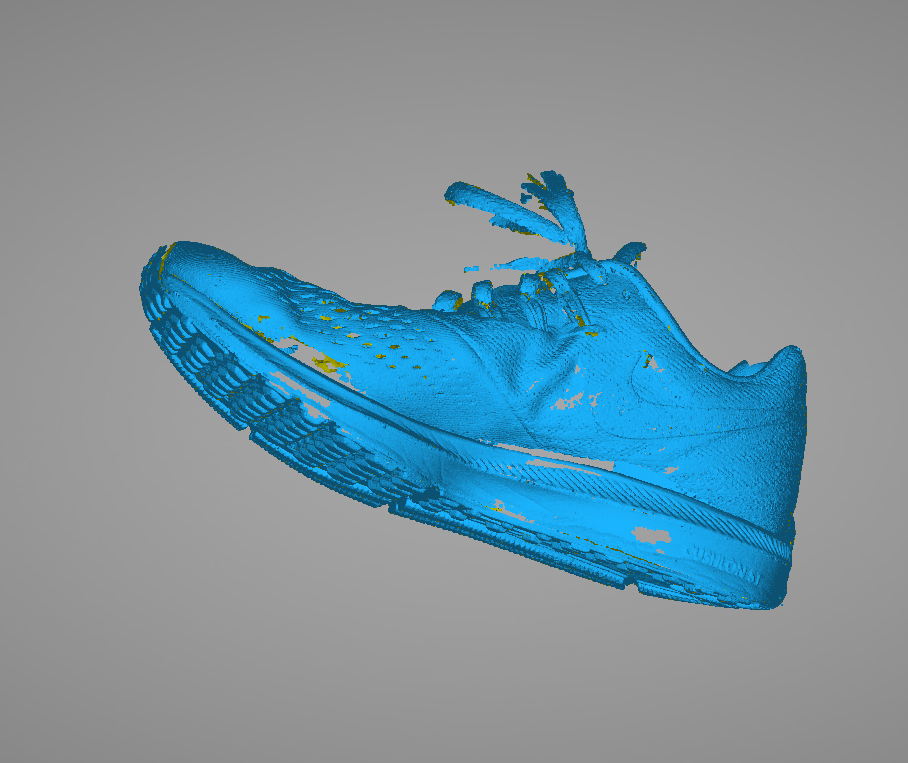
\includegraphics[width=6cm]{Shoe_Side}
\caption{Final Rough Scan}
\label{Image 25}
\end{figure}

\newpage

20. Select the mesh icon from the left tool bar (Figure 26). Then select "Unwatertight model" (Figure 27). Select Apply when prompted.

\begin{figure}[!htp]
\centering
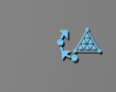
\includegraphics[width=6cm]{Meld}
\caption{After the scan has been completed, select the mesh key.}
\label{Image 26}
\end{figure}

\begin{figure}[!htp]
\centering
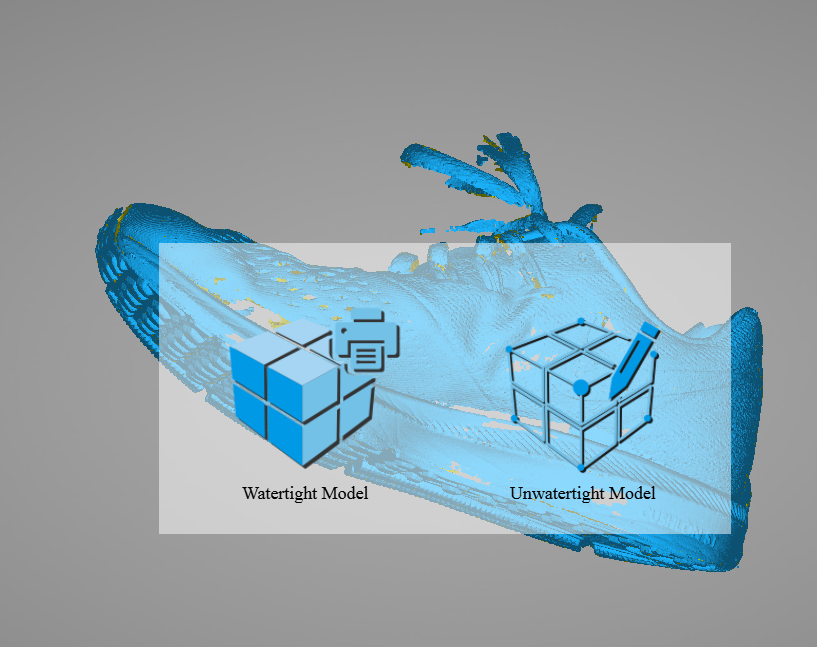
\includegraphics[width=6cm]{WAter}
\caption{Select "Unwatertight model"}
\label{Image 27}
\end{figure}

\newpage


21. After the final model has been generated (Figure 28), save it to the correct location as an STL file. 

\begin{figure}[!htp]
\centering
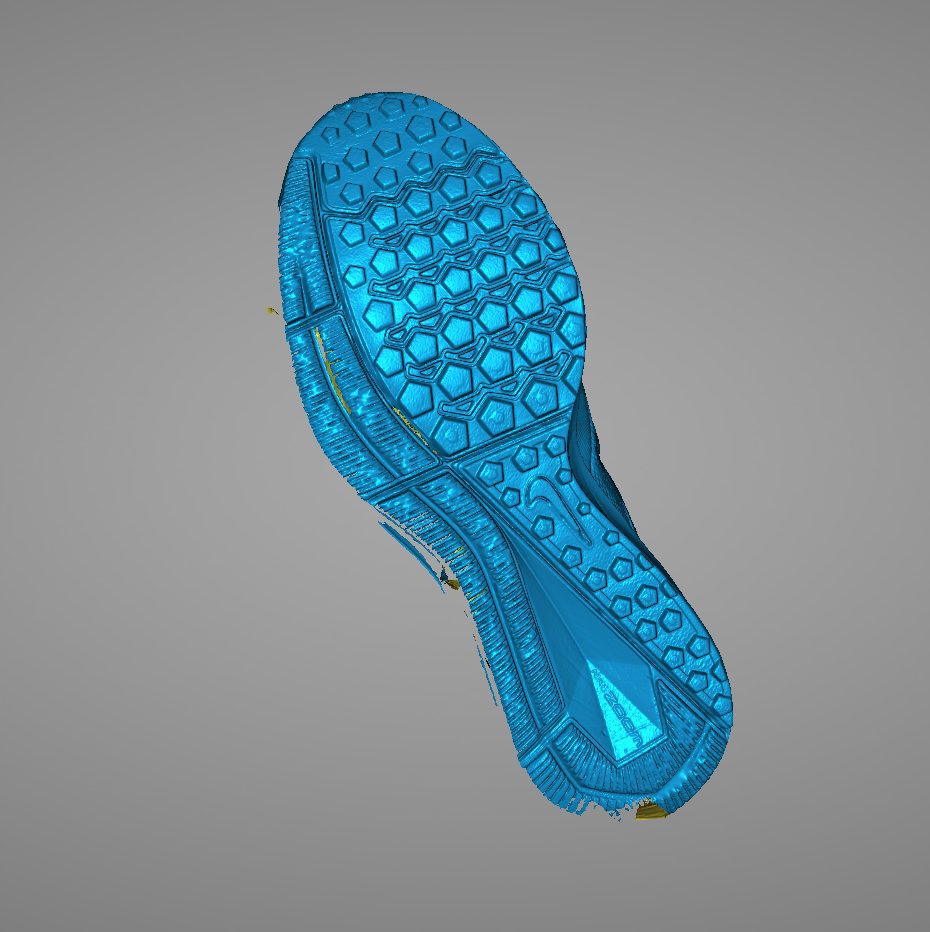
\includegraphics[width=6cm]{Final}
\caption{Final Model}
\label{Image 28}
\end{figure}

\end{document}
